\documentclass[a4paper,11pt]{report}
\usepackage[T1]{fontenc}
\usepackage[utf8]{inputenc}
\usepackage{lmodern}
\usepackage{graphicx}
\graphicspath{ {./images/} }



\title{SPE: CW2: Performance Modelling}
\author{Efe Ovadje (K1763735), Robert Cook (K1763733), Emmanuel Buraimo (K1630440)}
\date{2020}

\begin{document}

\maketitle
%\tableofcontents

\chapter*{Introduction}
We have been commissioned
by a financial services company,
to assess the feasibility of a system migration of a
legacy mainframe to the more recent Sun Solaris and
J2EE platform, while providing the expertise and guidance necessary.

A new application titled, 'Payments and Clearing' is expected to
utilize this new system.
It receives payments via \textit{http} from three separate business channels.
The application is comprised of four major components.
These are \textit{Inbound}, \textit{Message processing},
\textit{Processing and exception management} and the \textit{Oracle Server}.

The primary KPS identified during the performance and
scalability assessment was 'Process Peak Hour Current Processing Day Payments'.
There are two NFR's for this application,
'File Inter Arrival Time secs' (NFR1) and
'File 95 th Response Time secs' (NFR2).

\chapter*{Modelling}
This chapter details the layout and the functionality of the models, how they were created and their function along with the data we extracted from each individual model. The four main models defined here are the 
\begin{itemize}
  \item Inbound
  
  \item Message processing
  
  
  \item Processing and exception management (PEM)
  \item Oracle server
\end{itemize}


\section*{Inbound}
The inbound processing component receives payment submission files via HTTP, performs some technical validation on each payment via the MP. If there is an exception raised, this is rolled up into a referral via PEM, while the successful payments are placed into a single batch file which will be validated and distributed accordingly. Our model involved us creating a basic component for the inbound processing whose link to the interface allows us to receive the submission files. Within the basic component we have a SEFF which when opened writes a BLOB to the oracle server then internally does validation for 100 CPU cycles after which we modelled a loop action to iterate over every payment in the submission file. If an error occurred during this process, then we create a referral via PEM using an external call action. All this takes place within a branch action. 


\section*{Message processing}

The message processing component was part of an interconnected pair of other components that tightly functioned together 



\section*{Processing and exception management (PEM)}


\section*{Oracle server}
The Oracle server provided read and write functions that could access and manipulate application data, this was through the implementation of five procedures. These procedures are then accessed through the different application components, namely; Inbound Processing, Message Processing and PEM.\linebreak

When we started the project, the basic architecture of the Oracle server had been implemented. Our task was to build upon this architecture and model how the payment system used the Oracle server when a file was submitted into the system. Within the Oracle server Interface, we created the five procedures that would provide the necessary functionality. Connected to the Oracle Server Interface was a module named "Basic Component". The purpose of this component was to be able to assign specifically the action and the resource demand that each procedure would have. Through the use of SEFF diagrams, we could visually see how the different procedures would act and their resource consumption.

Based on the project brief that we were given, we modelled each procedure as follows; Procedure 1 had a resource demand of 500 CPU cycles per read business rules action from Oracle table 1, and an HDD of 2KB; Procedure 2 had a resource demand of 500 CPU cycles per write payment data action to Oracle table 2, and an HDD of 1KB; Procedure 3 had a resource demand of 2000 CPU cycles per backup of submission file action, and an HDD of 10MB; Procedure 4 had a resource demand of 50 CPU cycles per write exception action, and an HDD of 1KB; lastly Procedure 5 had a resource demand of 50 CPU cycles per write exception referral action, and an HDD of 1KB. 

\chapter*{Simulation}
Now that we had established our models within the repository, we
began to run simulations based on the specified resource environment.
Each resource environment is configured to run as an actual physical server. In this instance there are three servers. One for the Inbound component, another for the MP (Message processing) and PEM (Processing and Exception Management) and the last one for the Oracle DB.

As required we created two separate simulations 'SPESIM1' and
'SPESIM2' which differ by their key performance scenarios.

\begin{itemize}
\item Server 1: Inbound: CPUs: 12, CPU GHZ: 2
\item Server 2: MP, PEM: CPUs: 8, CPU GHZ: 2
\item Server 3: Oracle Server: CPUs: 16, CPU GHZ: 4
\end{itemize}

\section*{SPESIM1}
For the first simulation we conducted tests with a variable number of payments. First we ran a simulation using the number of elements as 100,1,000 and 10,000.
Below are the images from the respective runs along with their values.
\begin{figure}[hbtp]
\caption{Histogram of simulation 1 with number of elements as 100}
\centering
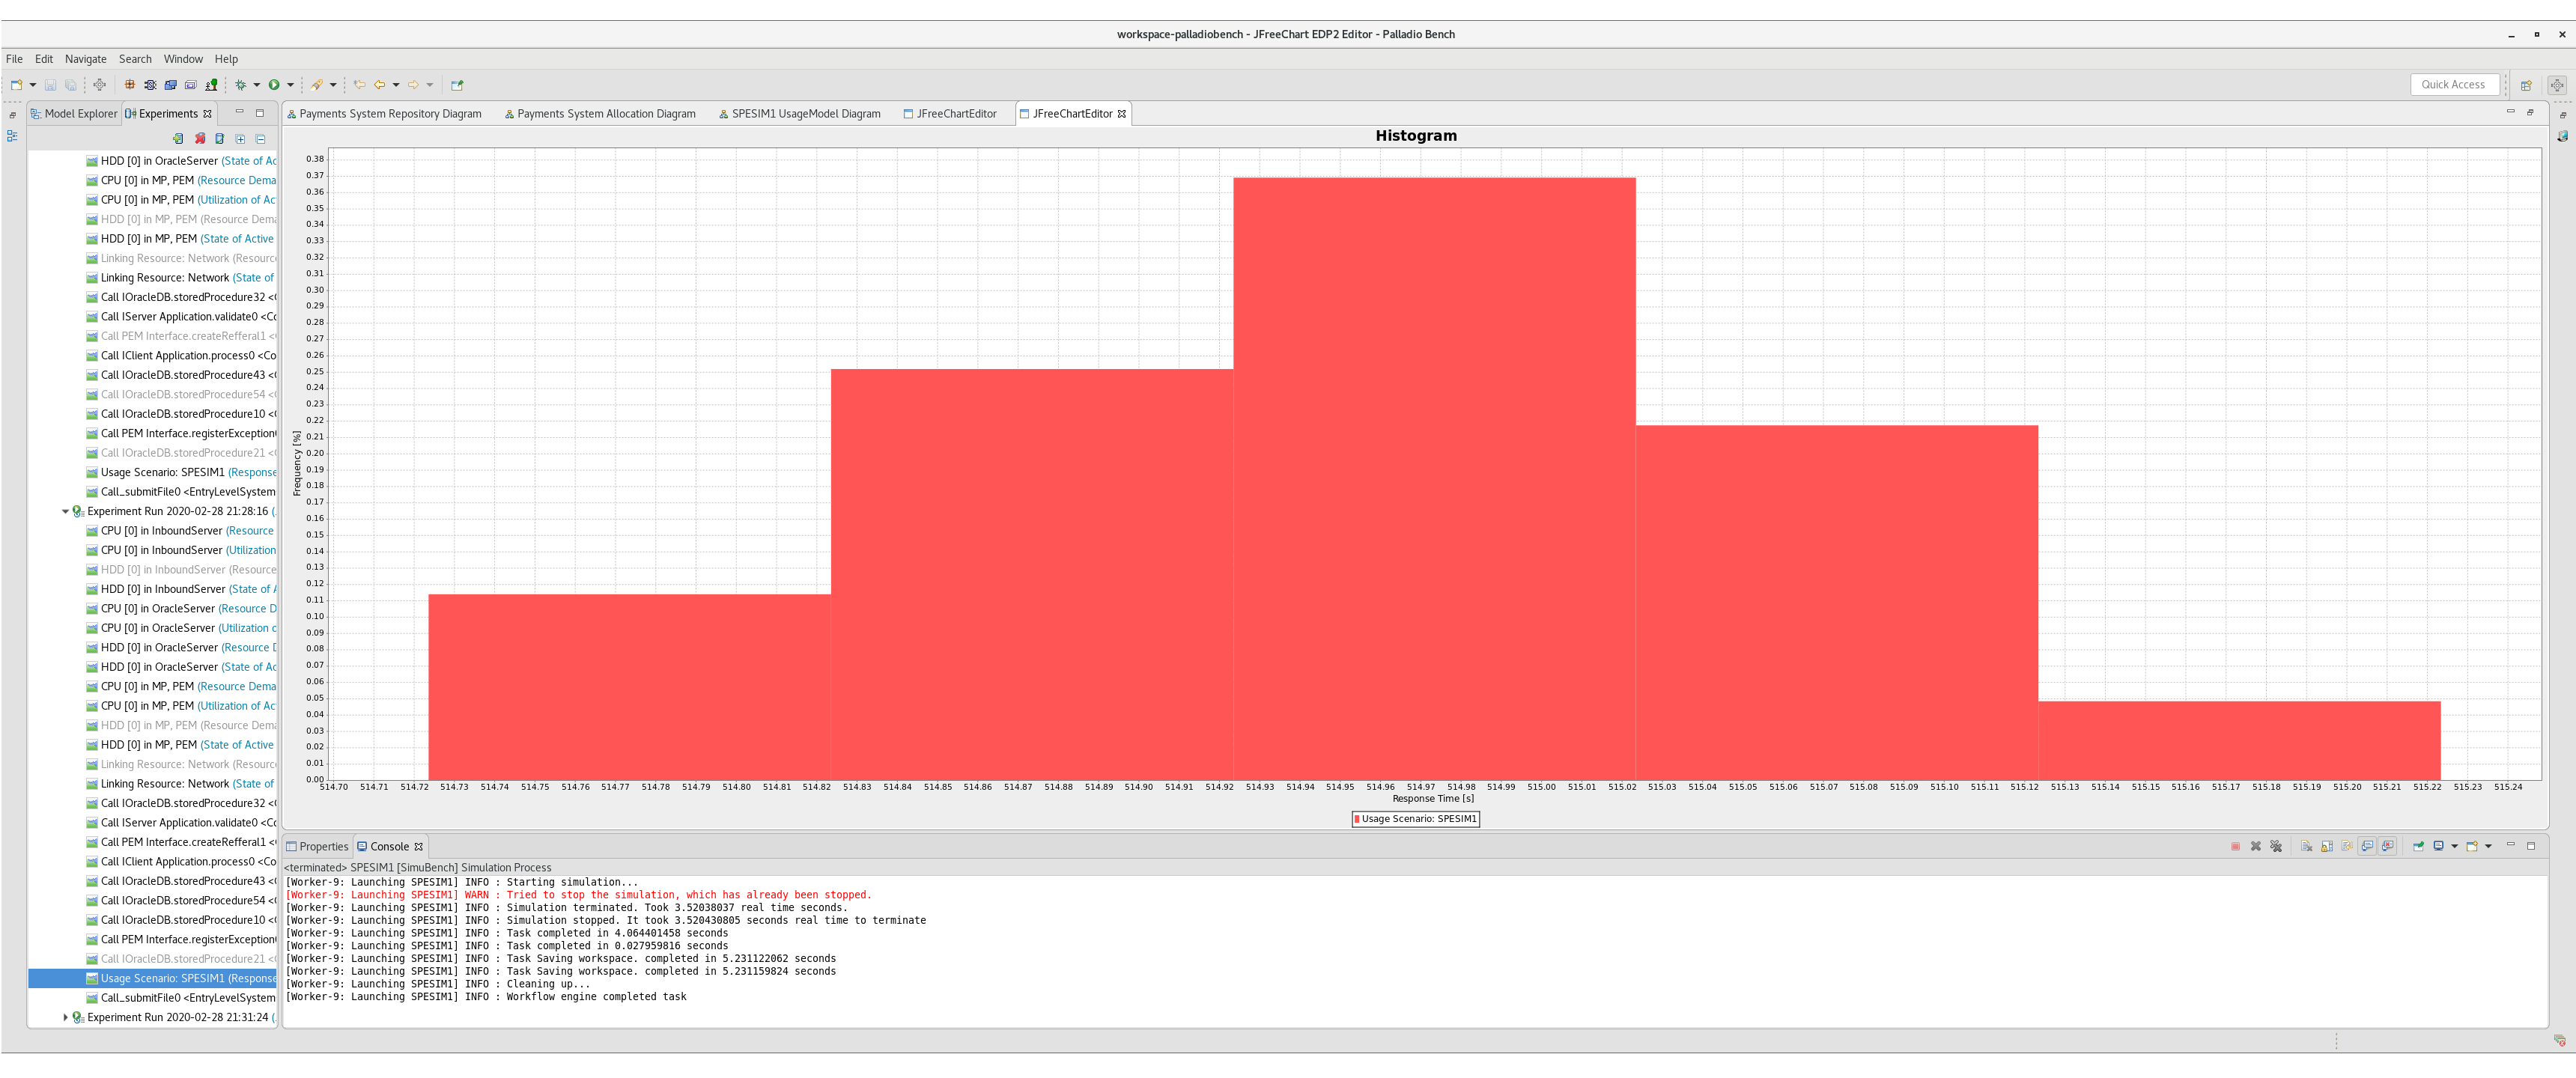
\includegraphics[width=160mm,scale=0.5]{../../../../../Pictures/sim1/hist.png}
\end{figure}

\begin{figure}[hbtp]
\caption{Cumulative distribution function (CDF) of simulation 1 with number of elements as 100}
\centering
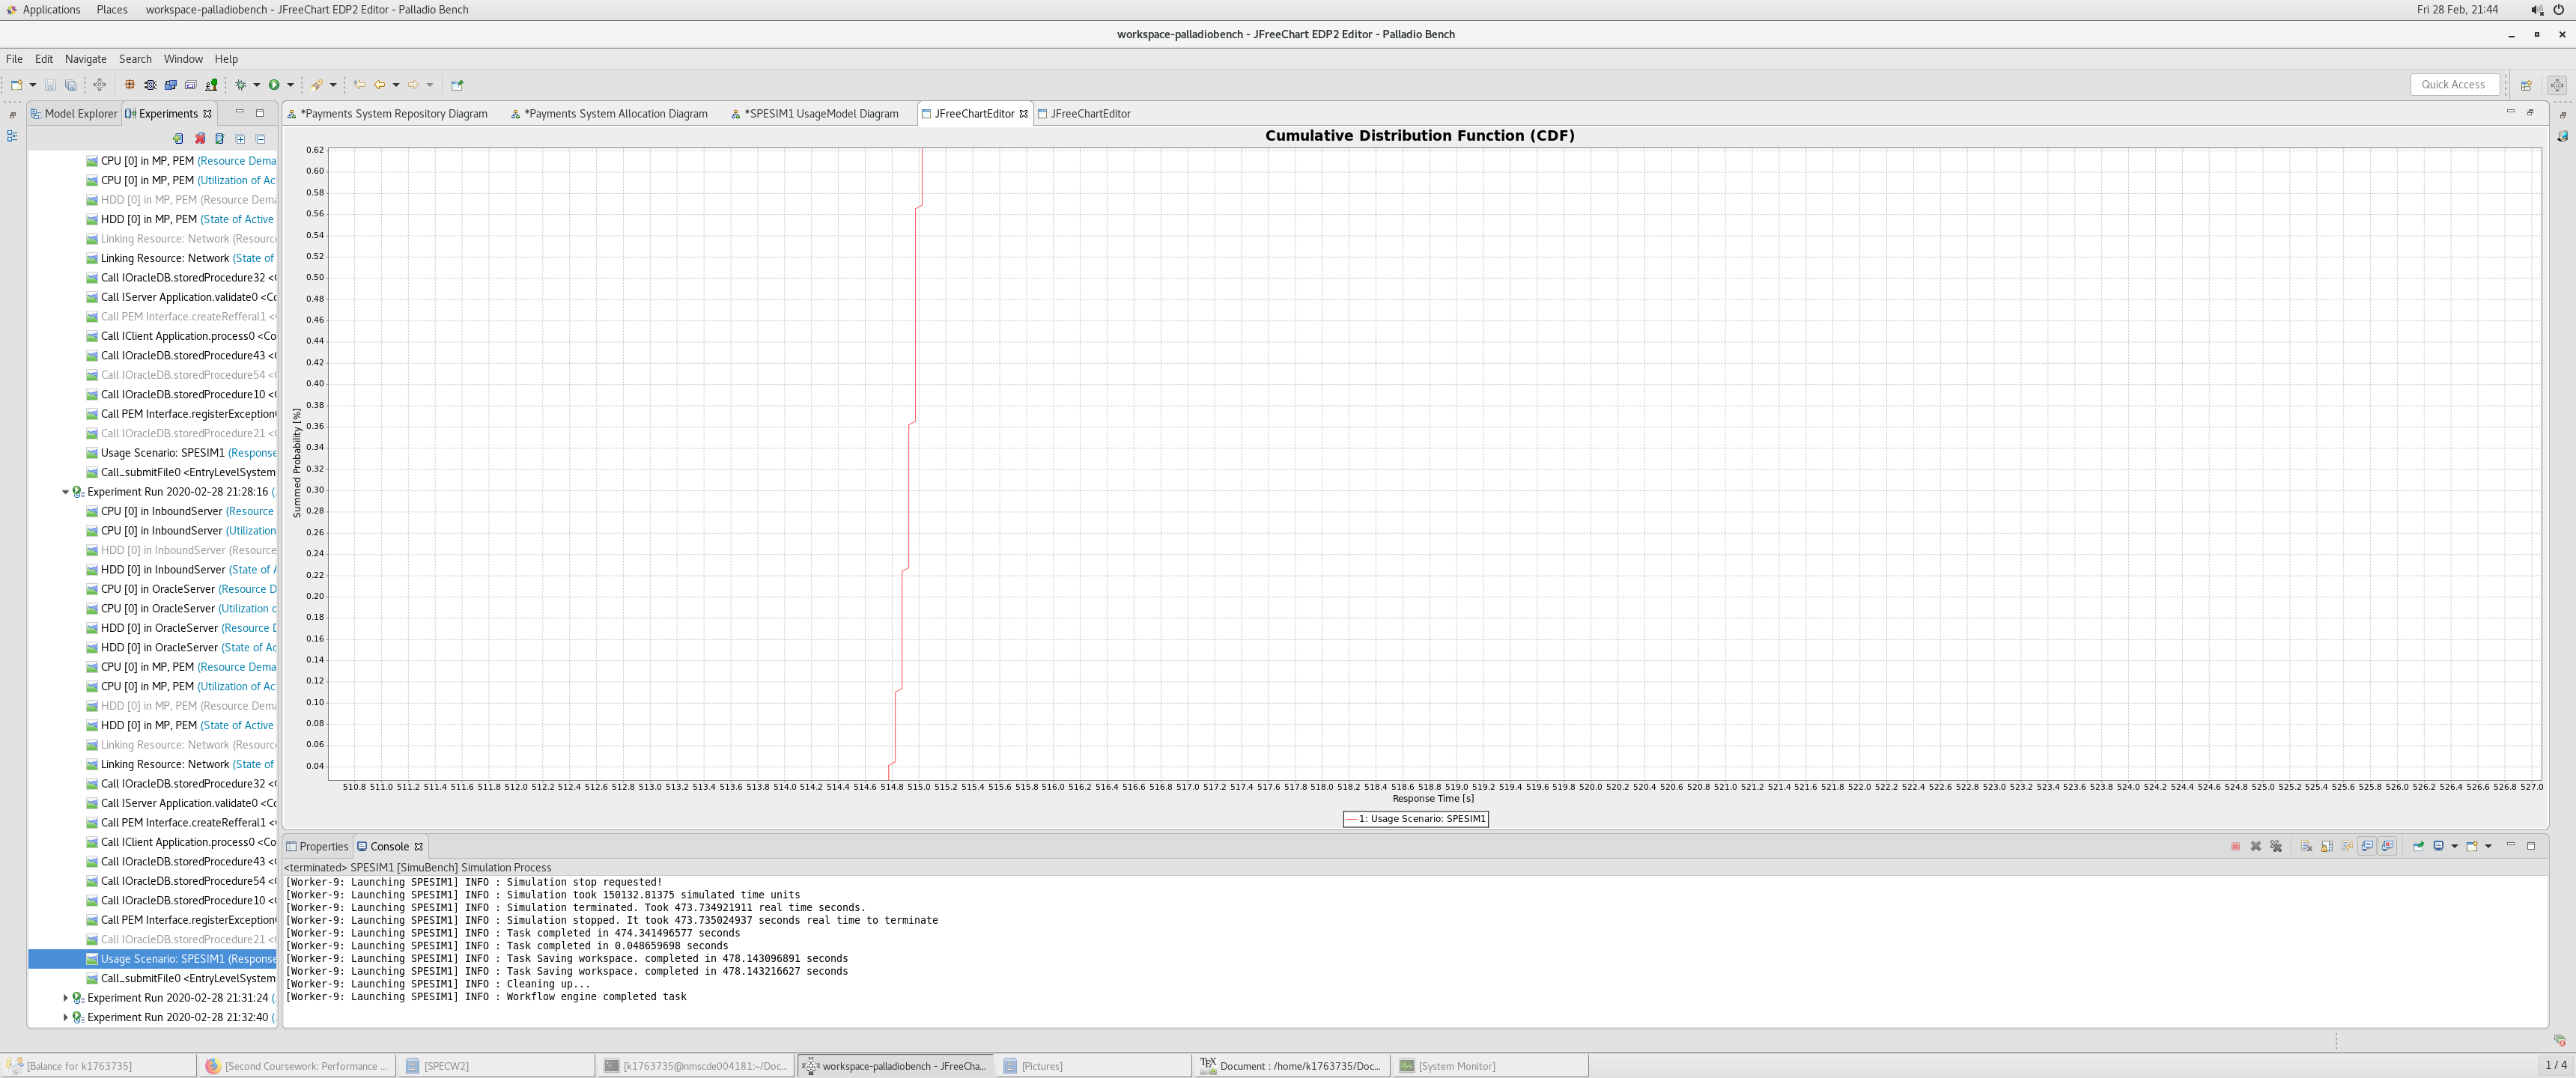
\includegraphics[width=160mm,scale=0.5]{../../../../../Pictures/sim1/cdf.png}
\end{figure}

\section*{SPESIM2}

%\chapter*{JMS modelling}

\end{document}
